Aprendizado de máquina (ou \textit{Machine learning} - ML) é uma sub área da inteligência artificial voltada à otimizar critérios de desempenho de acordo com análise de dados e ocorrências passadas \cite{alpaydin2010}. Uma das características mais marcantes da ML é a análise de conjuntos de dados para automatizar o desenvolvimento de modelos analíticos para suas funcionalidades, isso quer dizer que de acordo com essas análises e com dados de ocorrências já conhecidas por uma aplicação baseada em ML, o aprendizado possibilita às aplicações reagirem de maneira autônoma à eventualidades para as quais não foram programadas. Aprendizado de máquina normalmente é utilizado em duas situações que podem ser enxergadas pela análise do problema \cite{shalev2014}:

\begin{itemize}
    \item Complexidade elevada do problema: \\ Por exemplo, tarefas rotineiras que seres humanos executam, mas que para serem programadas o algoritmo teria uma complexitade enorme como dirigir ou reconhecer imagens. Outro exemplo é a necessidade de um processamento de uma massa de dados muito grande.
    \item Necessidade de adaptabilidade do sistema: \\ Por exemplo, detecção de diversos tipos de \textit{spam}, para marcar mensagens. \\
\end{itemize}

\subsection{Fluxo de trabalho}
    O fluxo de trabalho básico de ML consiste em duas fases, isto é, a de construção de um modelo e a de predição. Na primeira são utilizados dados históricos (ou dados de treinamento) para um ciclo de modelagem onde será definido, evoluido e otimizado um modelo de dados para que será utilizado para alimentar o algoritmo, realizando assim um tipo de aprendizado como mostrado na Figura 6. É a partir deste modelo otmizado que o algoritmo vai conseguir fazer predições sobre novos dados ou ainda categorizações \cite{brink2015}.

    \begin{figure}[ht]
            \centering
            \label{fig06}
                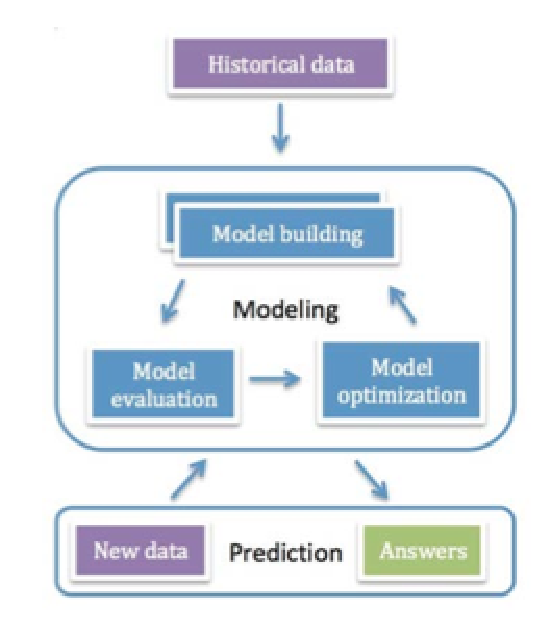
\includegraphics[keepaspectratio=true, scale=0.7]{editaveis/images/mlworkflow.eps}
            \caption{\textit{Workflow} básico de ML.}
            Fonte : Adaptado de \cite{brink2015}
    \end{figure}

\subsection{Tipos de aprendizado}
    \begin{itemize}
        \item Supervisionado: No aprendizado supervisionado, uma massa de dados de treinamento é consumida pelo programa possuindo \textit{labels} características que as classificam. Além disso, no momento em que um novo dado aparece sem essa \textit{label} (dado de teste), espera-se que o programa seja capaz de predizer qual a classificação do dado \cite{brink2015}.
        \item Não Supervisionado: No aprendizado não supervisionado, a massa de dados de treinamento é a mesma dos dados de teste, pois estes dados não possuem \textit{labels} que distinguem características. Dessa forma o programa reconhece as características a cada novo dado entregue e começa a fazer a separação de forma autônoma \cite{chao2011}.
        \item Reforço: No aprendizado por reforço, o programa ao receber um sinal de entrada dispara uma ação que muda o valor deste sinal. Assim que o valor do sinal de entrada é alterado e devolvido, mudando assim o estado do ambiente de aprendizagem. A partir disso é recebida uma nova entrada para disparar outra ação que novamente devolverá um valor diferente alterando o estado do ambiente, com a intenção de sempre se aumentar os valores de interação \cite{kaelbling1996}.
    \end{itemize}

% \subsection{Seleção de Características}
%     Segundo \cite{Yu2005}, seleção de características é o processo de seleção de um subconjuntos de características a partir de um conjunto original e a optmicidade desta seleção é me dida a partir de um critério de avaliação. Um processo de seleção de características é dividido em quatro fases:

%     \begin{itemize}
%         \item Definição de um subconjunto;
%         \item Avaliação do subconjunto;
%         \item Aplicação do critério de avaliação;
%         \item Validação do resultado.
%     \end{itemize}

%     A seleção de características é de suma importância para a aplicação de um modelo de aprendizado de máquina, pois é a partir de um bom subconjunto de características que resultados mais precisos são encontrados.

%     \subsection{Modelos de Seleção de Características}
%         Segundo \cite{Yu2005} os métodos de seleção de características são divididos em três tipos diferentes: modelo de filtro, modelo de envelopamento e o modelo híbrido.

%         O modelo de filtro seleciona o subconjunto de características a serem usadas utilizando-se basicamente das próprias características, sem a utilização de um algorítmo de seleção. Isso o torna computacionalmente mais eficiente, principalmente para extração de subconjuntos de características de bases de dados muito extensas.

%         O modelo de envelopamento utiliza um algorítmo pré determinado para a seleção do melhor subconjunto de características possível, e para garantir que o subconjunto escolhido seja o melhor possível, o modelo utiliza-se de um classificador próprio que avalia cada subconjunto gerado. Dessa forma o modelo de envelopamento é computacionalmente mais caro e lento conforme o tamamnho do conjunto de dados iniciais aumenta, porém este método garante melhoras resultados.

%         O modelo híbrido, combina os modelos de filtro e envelopamento para tentar extrair a melhor característica de cada um. Sendo assim, o modelo híbrido utiliza-se da generalização proposta no modelo de filtro para extrair um primeiro subconjunto, ainda grande de características, para redução do espaço de pesquisa e em seguida aplica o classificador utilizado no modelo de envelopamento para a partir daí conseguir um novo subconjunto menor e otimizado. \cite{Sutha2015}

%     \subsection{Método de seleção a ser aplicado}

%         O método de seleção a ser aplicado será o \textit{Linear Forward Selection}. Este método utiliza o modelo de seleção de envelopamento e o algorítmo \textit{sequential forward generation} para realizar a busca de características que irão integrar o subconjunto.

%         Este metodo funciona ranqueando todas as características, segundo alguma medida pré determinada, e construindo N subconjuntos a partir das características melhores ranqueadas. Por exemplo, a característica A$_1$ foi a melhor ranqueada, seguida por A$_2$ e A$_3$. Neste caso os subconjuntos S$_n$ a serem construídos serão dados da seguinte forma: S$_1$ {A$_1$}, S$_2$ {A$_1$, A$_2$}, S$_3$ {A$_1$, A$_2$, A$_3$} e a ssim por diante conforme a quantidade de características.

%         A partir daí, é feita a avaliação de cada subconjunto de acordo com algum classificador, e o subconjunto melhor ranqueado será o escolhido. Este método, por trabalhar a exaustão na busca de subconjuntos apresenta o melhor subconjunto possível, em detrimento de uma eficiência computacional baixa e de um tempo de resposta mais alto em relação a outros métodos.\cite{Franco2015}